\DylanSpeak
\subsection{Présentation du projet}
\begin{frame}{Le projet BandStorm}
	\begin{itemize}
		\item Réseau social pour amateurs de musique
	\end{itemize}
	\vfill
	\begin{block}{Différentes fonctionnalités}
		\begin{itemize}
			\item Poster des statuts
			\item Suivre des utilisateurs
			\item Rejoindre des groupes
			\item Créer des événements
		\end{itemize}
	\end{block}
\end{frame}

\JulianSpeak
\subsection{Agilité}
\begin{frame}{Méthode Scrum}
\begin{figure}
\centering
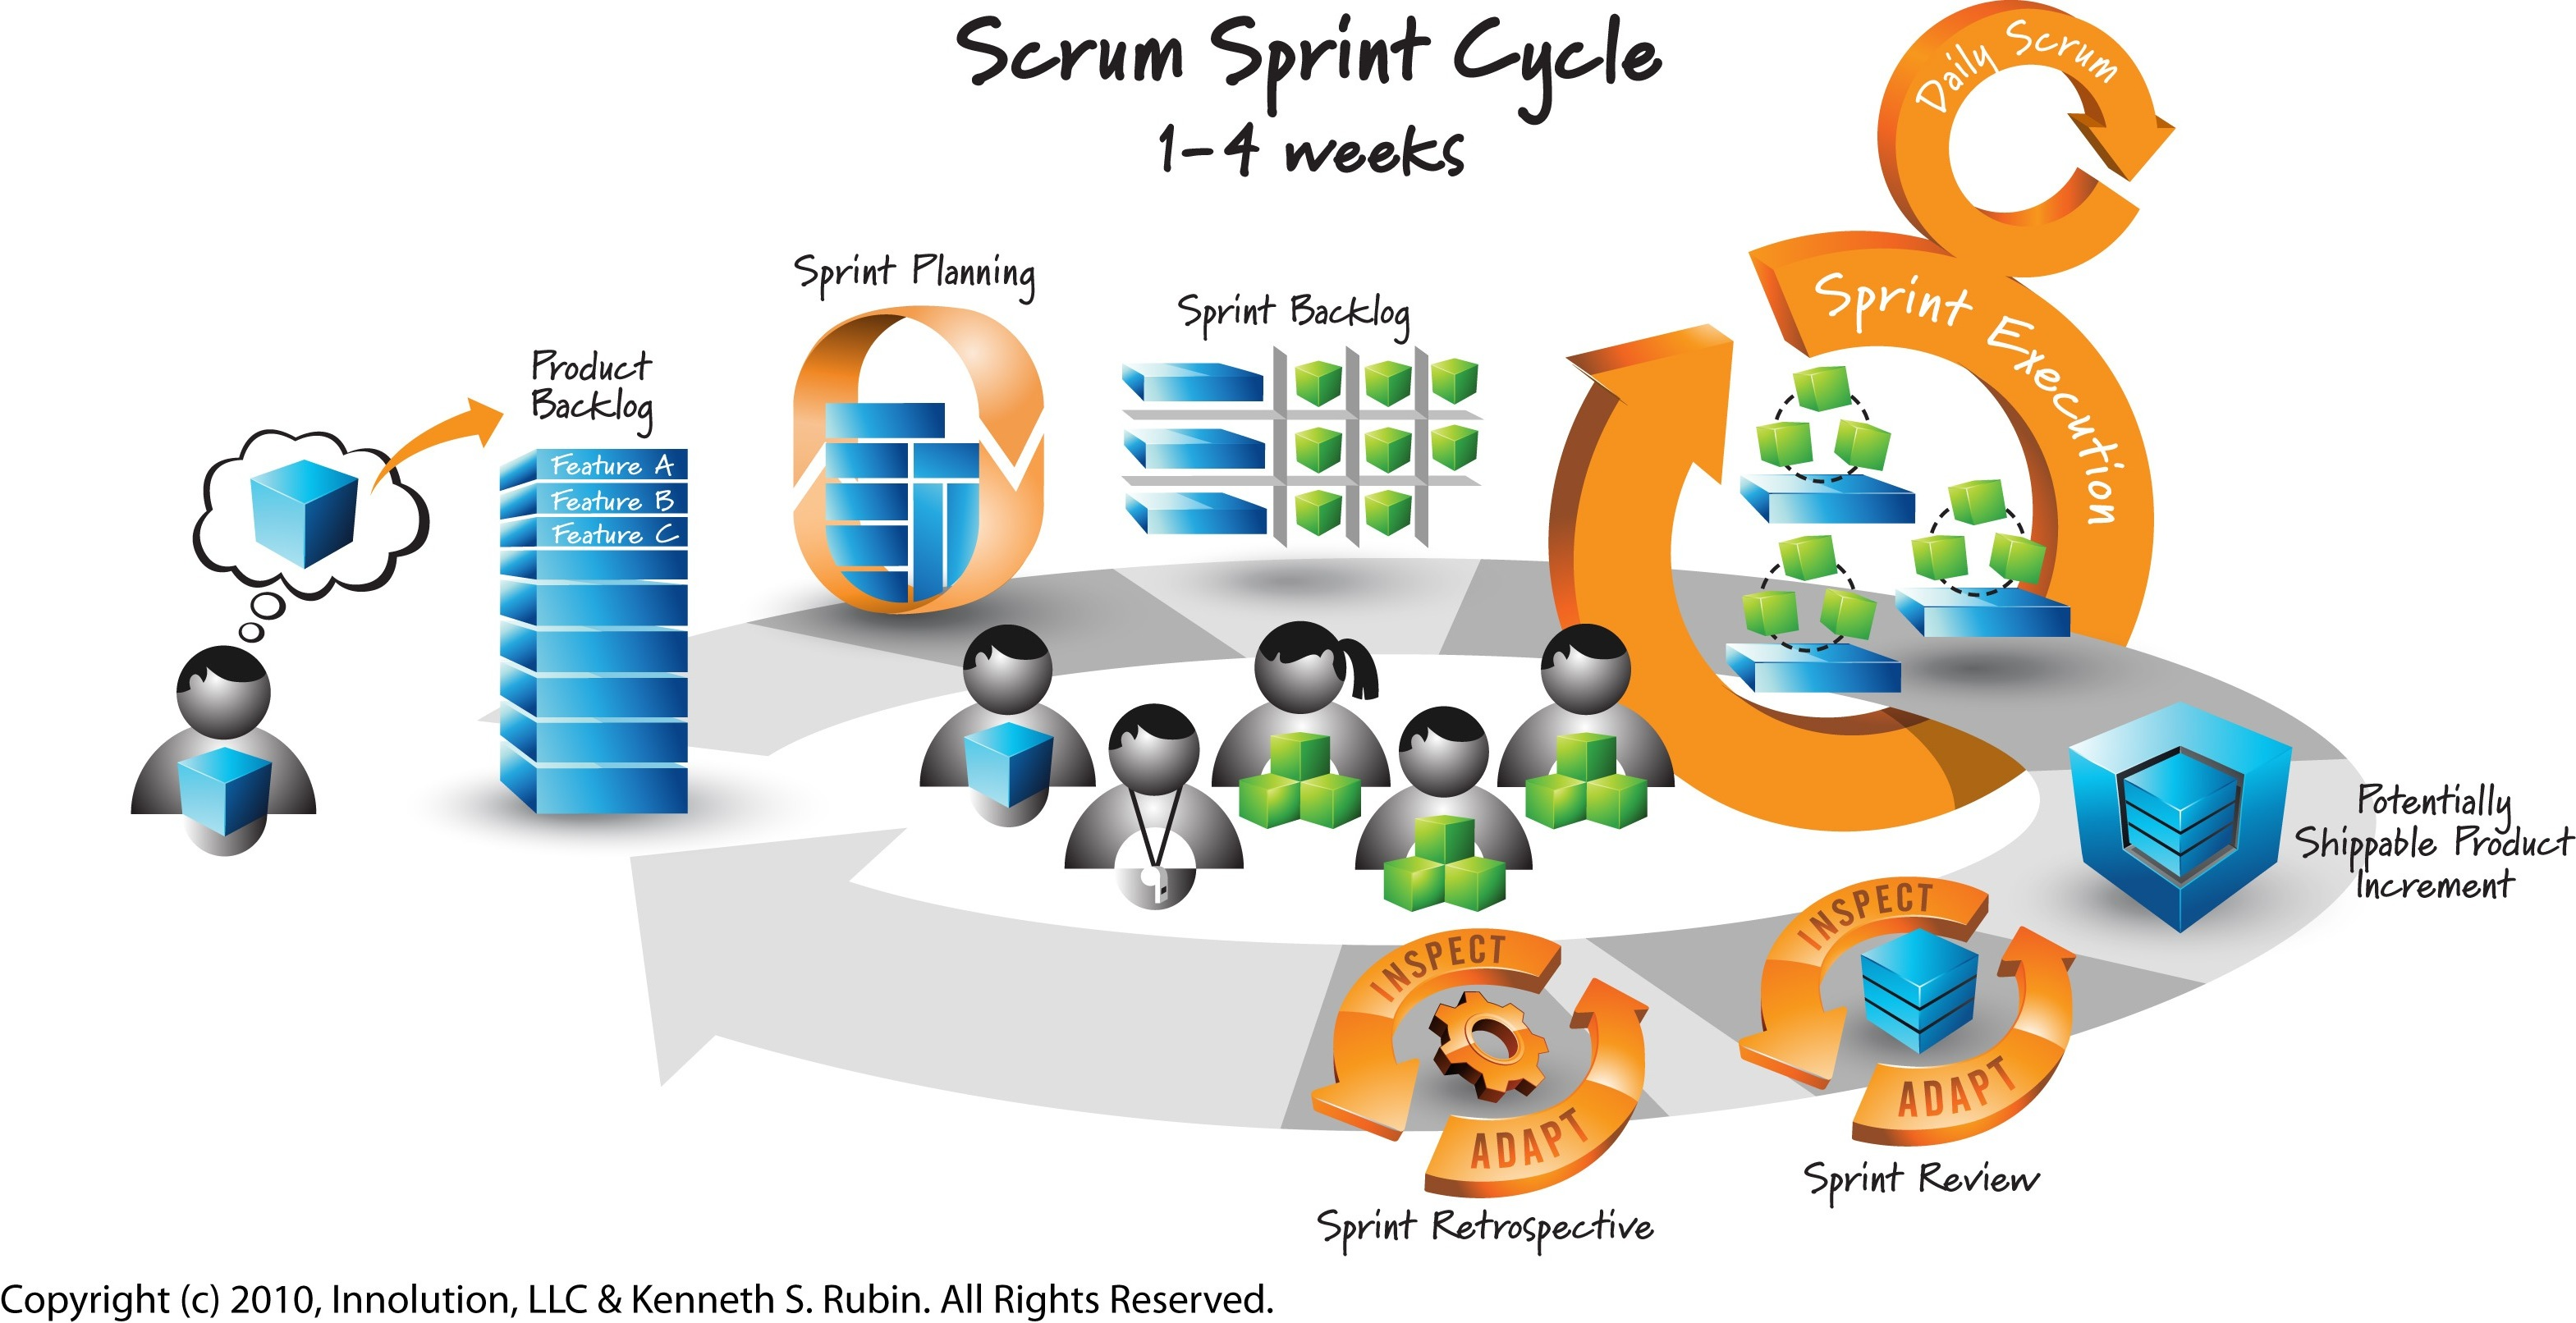
\includegraphics[width=\linewidth]{images/projectManagement/scrum}
\caption{Fonctionnement d'un Sprint avec Scrum}
\label{fig:scrum}
\end{figure}
\end{frame}

\begin{frame}{Définition de << fini >>}
	Une \textit{story} est finie si : 
	\vspace{-10px}
	\begin{itemize}
		\item Testée (unitaire et intégration)
		\item Couverture de tests en ligne \texttt{> 80\%}
%		\begin{itemize}
%			\item 100\% couverture (classes de modèles)
%			\item 80\% couverture (contrôleurs)
%			\item 80\% couverture (services)
%		\end{itemize}
		\item Tests d'acceptance validés (\textit{Product Owner})
		\item Build Travis CI \textit{passed}
		\item Pas de \textit{major} \texttt{Codenarc}
		\item Pas de \textit{major} \& \textit{critical} \texttt{SonarQube}
		\item Javadoc rédigée
	\end{itemize}
	\vfill
	\pause
	Lorsqu'une \textit{story} est terminée : 
	\vspace{-10px}
	\begin{itemize}
		\item Passage dans la colonne \textit{done}
		\item Fusion de la fonctionnalité dans la branche mère
	\end{itemize}
%		\item Branche pour l’issue GitHub
%		\item \textit{Pull request} revue (product owner)

%		\item 	Build Travis CI : OK
%		\item 	Codenarc : OK 
%		\item 	SonarQube : correction criticals & majors
%				\item Javadoc rédigée
%	Story → colonne “done”.
%	Fusion de la branche (story) dans la branche mère (Sprint).




\end{frame}
